\begin{figure}[htbp]
	\centering
	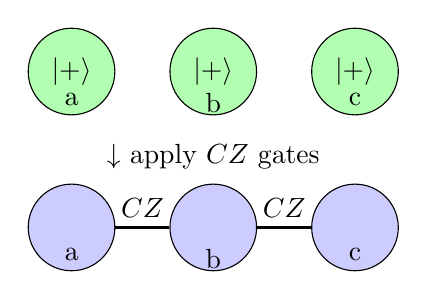
\begin{tikzpicture}[scale=0.9]
		\node[draw, circle, fill=green!30, minimum size=1.1cm] (a) at (0,0) {$|+\rangle$};
		\node[draw, circle, fill=green!30, minimum size=1.1cm] (b) at (2,0) {$|+\rangle$};
		\node[draw, circle, fill=green!30, minimum size=1.1cm] (c) at (4,0) {$|+\rangle$};

		\node[below=0.15cm] at (a) {a};
		\node[below=0.15cm] at (b) {b};
		\node[below=0.15cm] at (c) {c};

		\node[thick] at (2,-1.2) {$\downarrow$ apply $CZ$ gates};

		\node[draw, circle, fill=blue!20, minimum size=1.1cm] (a2) at (0,-2.2) {};
		\node[draw, circle, fill=blue!20, minimum size=1.1cm] (b2) at (2,-2.2) {};
		\node[draw, circle, fill=blue!20, minimum size=1.1cm] (c2) at (4,-2.2) {};

		\node[below=0.15cm] at (a2) {a};
		\node[below=0.15cm] at (b2) {b};
		\node[below=0.15cm] at (c2) {c};

		\draw[thick] (a2) -- node[above] {$CZ$} (b2);
		\draw[thick] (b2) -- node[above] {$CZ$} (c2);

	\end{tikzpicture}
	\caption{Construction of a graph state from a graph $G$. Each vertex represents a qubit initialized in $|+\rangle$, and each edge represents a controlled-$Z$ entangling operation applied between connected qubits. Graph State $|G\rangle$: Vertices = $|+\rangle$ qubits, Edges = $CZ$ applied.}
	\label{fig:graph-state-construction}
\end{figure}
